\documentclass[twoside,11pt]{article}

\usepackage{aa228-jmlr2e}
\usepackage{amsmath}
\usepackage{graphicx}
\usepackage{lipsum}
\usepackage{listings}
\usepackage{url}
\usepackage{cleveref}
\usepackage{subcaption}
\usepackage{tikz}
\usetikzlibrary{arrows.meta, positioning, calc}

\begin{document}

% More details can be found here: https://aa228.stanford.edu/final-project/
\title{Automating Parametric CAD Sketch Synthesis via Sequential Decision Making}
\newcommand{\shorttitle}{Automating CAD Sketches} 

%===========================================
% Fill in your names and emails
%===========================================
\name{Christopher Luey}
\email{christopherluey2025@u.northwestern.edu}

\maketitle

\section{Goal}
Modern mechanical design teams still spend significant time translating requirement tables into parametric computer-aided design (CAD) sketches that seed downstream solid modeling. I propose to automate the early-stage sketching of planar bracket components directly from structured requirement tuples by learning from the SketchGraphs subset of the Fusion 360 Gallery dataset, which provides 15{,}390 human-authored sketches with fully timestamped modeling operations, constraint graphs, and parameter values \citep{Willis2021Fusion360, SketchGraphs2020}. Focusing on L- and U-shaped brackets with at most 12 primitives focuses on exercising sequential decision-making tools on meaningful engineering constraints.

We have three deliverables: (i) Days 1--4: curate a bracket-focused dataset slice, extract feature statistics (primitive frequencies, constraint co-occurrence, dimensional ranges), and publish preprocessing notebooks; (ii) Days 5--9: train and validate a behavior-cloned policy that maps requirement tokens and partial sketches to the next CAD action, logging calibration metrics for downstream risk analysis; and (iii) Days 10--14: layer an uncertainty-aware action selection module (conservative Q-learning fine-tuning plus ensemble-based confidence scoring) and run ablation studies quantifying constraint satisfaction rate, sketch length, and solver success on a held-out specification set. Achieving these milestones will demonstrate that principled decision-making approaches can materially reduce iteration time in CAD automation while respecting design-engineering rigor \citep{Kochenderfer2022}.


\section{Decision Making}
I frame automated sketch construction as a partially observable Markov decision process (POMDP) in which each episode corresponds to building a parametric sketch that satisfies a requirement tuple $(g, c, d)$ containing desired geometry (hole pattern, flange lengths), hard constraints (mounting plane, thickness), and design intents (load directions). The latent state $s_t$ comprises the full canonical sketch graph, including primitive embeddings, unresolved constraint slack, and the latent ``style cluster'' inferred from SketchGraphs metadata (Autodesk provides eight unsupervised clusters covering structural, decorative, and mechanical sketches \citep{SketchGraphs2020}). The observation $o_t$ exposes the partial sketch graph available to the agent, requirement tokens, and noisy signals from the constraint solver (feasibility flags, residual norms).

The action space leverages SketchGraphs' taxonomy: five primitive types (line, arc, circle, point, spline) and nine constraint/dimension types (coincident, perpendicular, parallel, equal, tangent, horizontal, vertical, distance, angle) with parameter bins learned from empirical quantiles. Each action is factored into a discrete intent $a^{\text{type}}_t$ and continuous parameter vector $a^{\text{param}}_t$; the former is modeled as a categorical distribution, whereas the latter is sampled from Gaussian heads centered on dataset means with learned variance. Transitions $T(s_{t+1}\,|\,s_t, a_t)$ are deterministic under the CAD kernel but I model tolerance-related perturbations via a learned residual dynamics model that perturbs endpoints and constraint slack to mimic solver adjustments.

Rewards combine dense shape guidance with terminal feasibility checks. A $-0.05$ step cost encourages concise sketches, partial rewards score constraint satisfaction and similarity between generated and target dimensions (scaled Chamfer distance on anchor points), and a terminal bonus of $+1.0$ is granted when all hard constraints fall within tolerance bands. The hierarchical structure enables efficient planning: a high-level policy selects which substructure to extend (e.g., ``extend flange'') while a low-level controller chooses primitive parameters. Offline behavior cloning on filtered expert trajectories supplies the initial policy; uncertainty-aware improvement follows via conservative Q-learning and limited-horizon model-predictive control that rolls out candidate action sequences under the learned residual model.

\section{Sources of Uncertainty}
Three uncertainty sources dominate this problem. (i) \textbf{Demonstration variability:} SketchGraphs encodes multiple valid action permutations for similar brackets; some designers add driving dimensions before closing loops, others after. I will capture this epistemic uncertainty with a bootstrap ensemble of graph encoders and Q-heads, using disagreement as a risk metric. (ii) \textbf{Specification ambiguity:} Requirement tuples derived from handbooks may omit secondary dimensions (fillet radii, hole clearances). I will model the missing values as latent random variables with truncated Gaussian priors fit to the curated dataset slice and maintain beliefs $\beta_t$ that are updated whenever the solver reports infeasible constraints. (iii) \textbf{Solver stochasticity and tolerances:} Autodesk's constraint solver occasionally perturbs primitive endpoints when loops are nearly singular, effectively injecting action noise. I will emulate this aleatoric component through the learned residual dynamics model and propagate tolerance bands (e.g., $\pm 0.2$ mm for bolt-hole spacing) into the reward.

During training, Monte Carlo dropout and deep ensembles yield calibrated predictive intervals; conservative Q-learning uses the lower confidence bound to penalize risky actions. At deployment, the agent selects actions using a risk-sensitive criterion $\max_a \mathbb{E}[Q(s,a)] - \lambda \sqrt{\text{Var}[Q(s,a)]}$, where $\lambda$ is tuned on validation requirements to balance aggressiveness and robustness. Evaluation will report mean performance, $95\%$ confidence intervals, and worst-case outcomes conditioned on solver failures, providing a principled view of residual uncertainty.

\section{Sketches of Solution (Optional)}
\Cref{fig:decision-flow} depicts the closed-loop decision process the agent will implement, highlighting how specification parsing, belief updates, policy inference, and uncertainty handling interact with the CAD solver.

\begin{figure}[t]
    \centering
    \resizebox{0.92\linewidth}{!}{%
    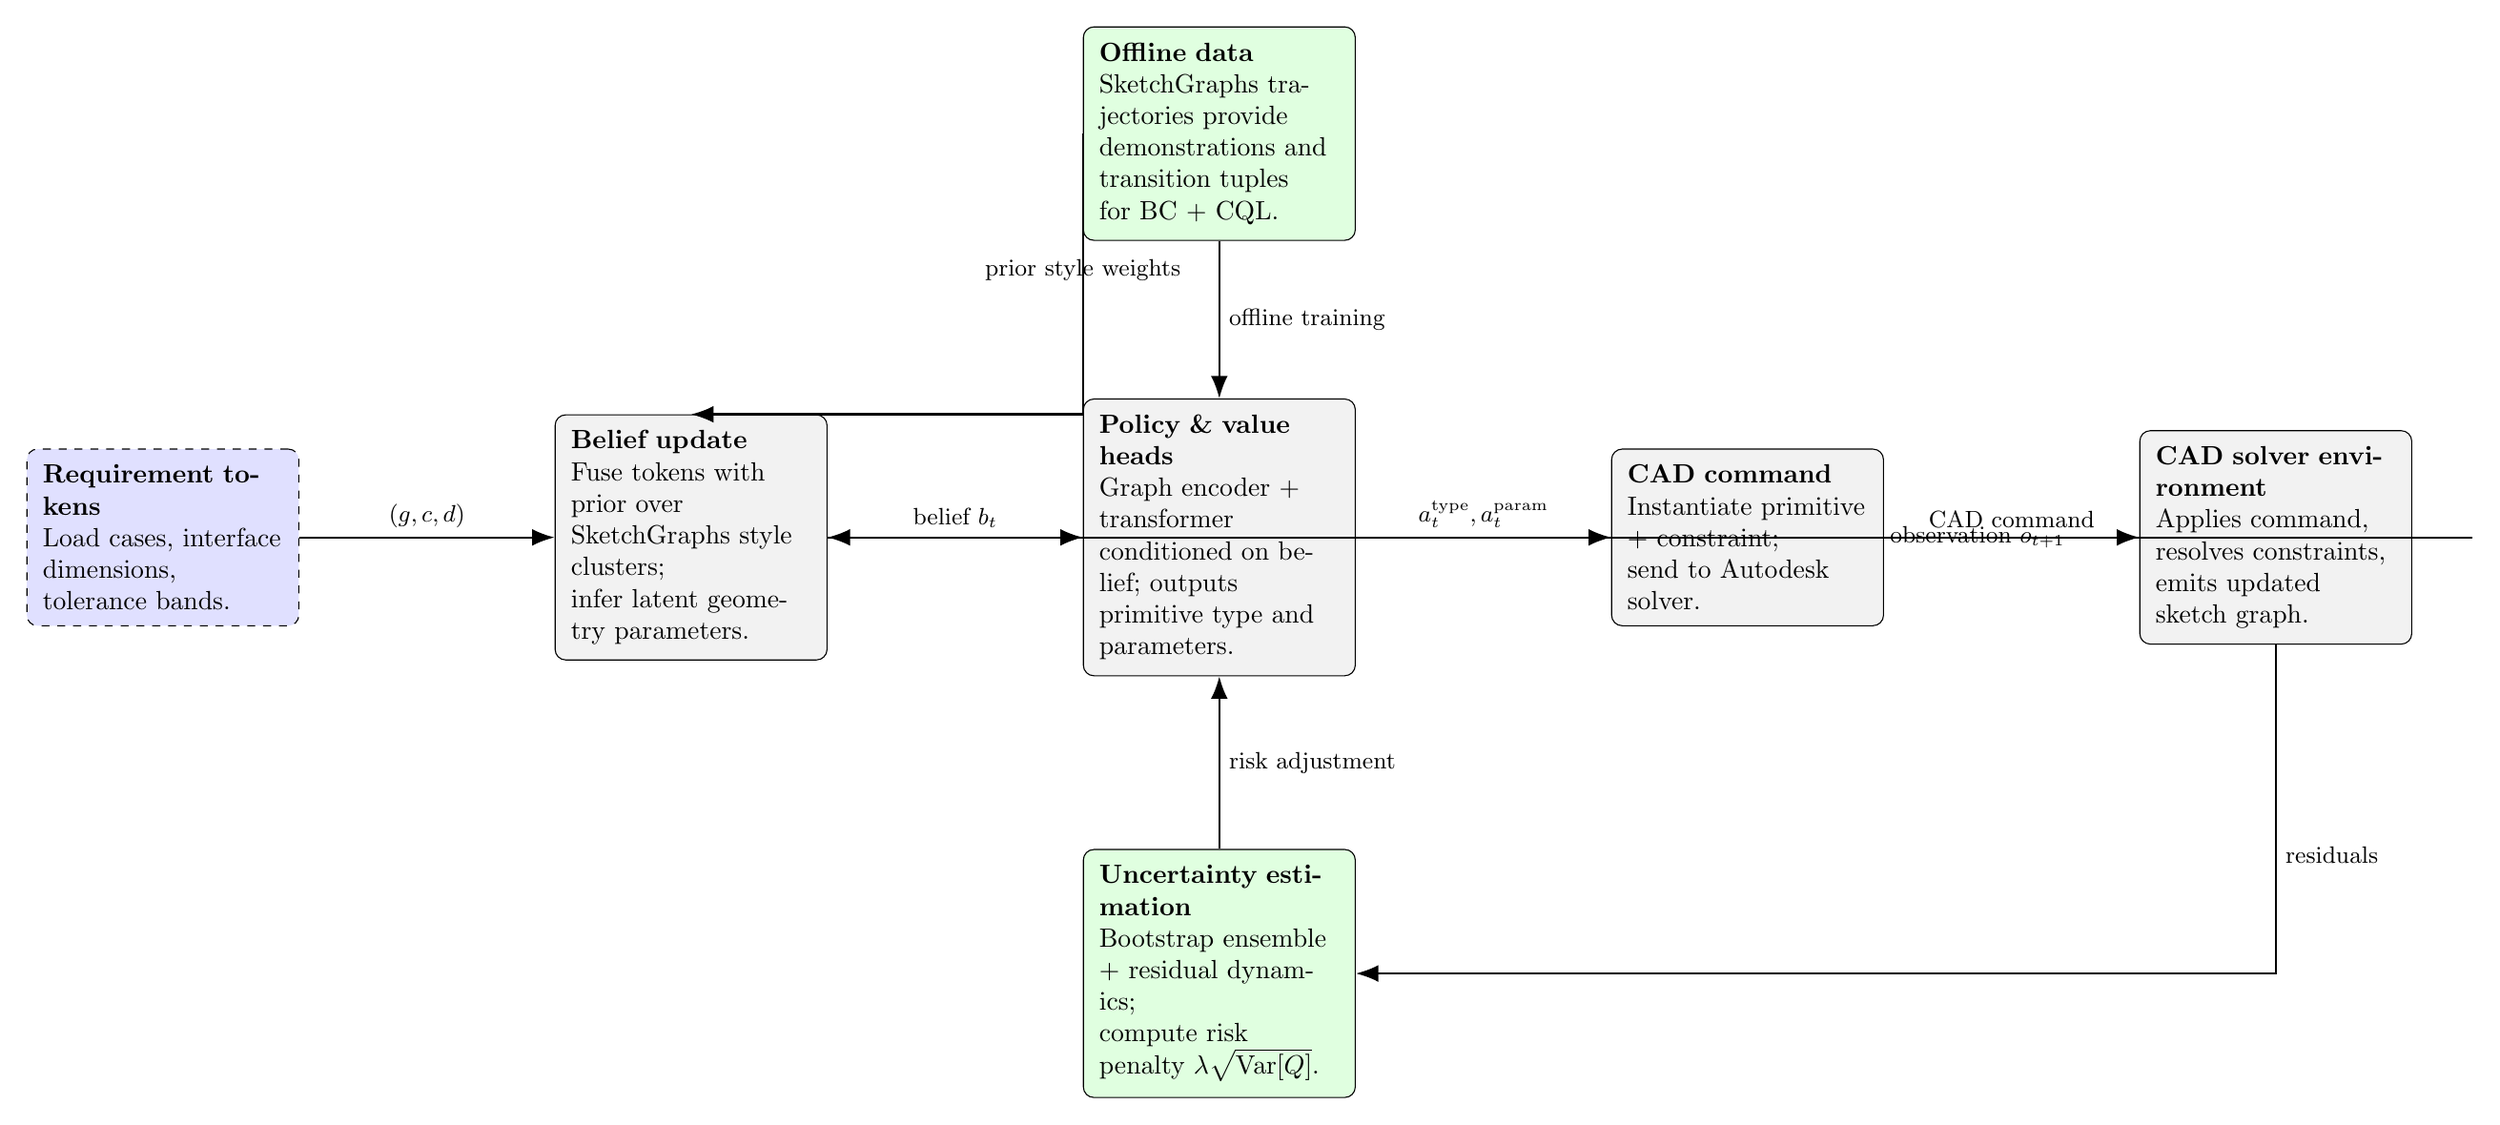
\begin{tikzpicture}[
        node distance=2.4cm,
        block/.style={rectangle, rounded corners, draw=black, align=left, minimum height=1.4cm, text width=3.2cm, inner sep=6pt, fill=gray!10},
        data/.style={rectangle, rounded corners, draw=black, align=left, minimum height=1.4cm, text width=3.2cm, inner sep=6pt, fill=blue!12, dashed},
        monitor/.style={rectangle, rounded corners, draw=black, align=left, minimum height=1.4cm, text width=3.2cm, inner sep=6pt, fill=green!12},
        arrow/.style={-{Latex[length=3mm]}, thick}
    ]
        \node[data] (spec) {\textbf{Requirement tokens}\\Load cases, interface dimensions,\\tolerance bands.};
        \node[block, right=3.4cm of spec] (belief) {\textbf{Belief update}\\Fuse tokens with prior over\\SketchGraphs style clusters;\\infer latent geometry parameters.};
        \node[block, right=3.4cm of belief] (policy) {\textbf{Policy \& value heads}\\Graph encoder + transformer\\conditioned on belief; outputs\\primitive type and parameters.};
        \node[block, right=3.4cm of policy] (action) {\textbf{CAD command}\\Instantiate primitive + constraint;\\send to Autodesk solver.};
        \node[block, right=3.4cm of action] (env) {\textbf{CAD solver environment}\\Applies command, resolves constraints,\\emits updated sketch graph.};
        \node[monitor, above=2.1cm of policy] (dataflow) {\textbf{Offline data}\\SketchGraphs trajectories provide\\demonstrations and transition tuples\\for BC + CQL.};
        \node[monitor, below=2.3cm of policy] (uncertainty) {\textbf{Uncertainty estimation}\\Bootstrap ensemble + residual dynamics;\\compute risk penalty $\lambda \sqrt{\mathrm{Var}[Q]}$.};

        \draw[arrow] (spec) -- node[above]{\small $(g,c,d)$} (belief);
        \draw[arrow] (belief) -- node[above]{\small belief $b_t$} (policy);
        \draw[arrow] (policy) -- node[above]{\small $a_t^{\text{type}}, a_t^{\text{param}}$} (action);
        \draw[arrow] (action) -- node[above]{\small CAD command} (env);
        \coordinate (feedback) at ($(env.east)+(0.8,0)$);
        \draw[arrow] (env.east) -- (feedback) |- node[pos=0.68,right]{\small observation $o_{t+1}$} (belief.east);
        \draw[arrow] (dataflow.south) -- node[right]{\small offline training} (policy.north);
        \draw[arrow] (dataflow.west) |- node[pos=0.28,above]{\small prior style weights} (belief.north);
        \draw[arrow] (uncertainty.north) -- node[right]{\small risk adjustment} (policy.south);
        \draw[arrow] (env.south) |- node[pos=0.32,right]{\small residuals} (uncertainty.east);
    \end{tikzpicture}
    }
    \caption{Algorithmic loop: requirements feed a belief-augmented policy trained on SketchGraphs; uncertainty estimates shape action selection before commands are executed in the CAD solver, whose feedback updates both belief and risk models.}
    \label{fig:decision-flow}
\end{figure}

% References
\bibliography{references}


\end{document}
